 %\title{Landscape Brochure Template}
 % This example is from http://www.ctan.org/tex-archive/macros/latex/contrib/flowfram/
 

\documentclass[a4paper, 11pt]{report}
\usepackage{amsmath}
\usepackage[landscape,margin=1in]{geometry}
\usepackage{color}
\usepackage{flowfram}
\usepackage[colorlinks]{hyperref}
\usepackage{indentfirst}
\usepackage{graphicx}
\usepackage{csquotes}
\usepackage{setspace}

\renewcommand{\baselinestretch}{1.2} 

\newenvironment{myboxed}
    {
        \begin{center}
        \begin{tabular}{p{0.7\textwidth}}
        \hline\
    }
    { 
        \\\hline
        \end{tabular} 
        \end{center}
    }


\renewcommand{\familydefault}{cmss}

\adjustheight{\textheight}

\onecolumninarea[1-100]{0.7\textwidth}{\textheight}{0.3\textwidth}{0pt}
%\twocolumninarea[>3]{0.8\textwidth}{\textheight}{0.52\textwidth}{0pt}


\newdynamicframe{0.3\textwidth}{0.7\textheight}{0pt}{0pt}[left]

\dfchaphead*{left}
\renewcommand{\DFchapterstyle}[1]{%
\raggedright\Huge\slshape\MakeUppercase{#1}\par}

\vtwotone[1]{0.3\paperwidth}{[cmyk]{0.37,0,0.07,0.50}}{backleft}%
{0.7\paperwidth}{[cmyk]{0.37,0,0.15,0.32}}{backright}

\vtwotonetop{1cm}{0.3\paperwidth}{[cmyk]{0.37,0,0.07,0.50}}{topleft}%
{0.7\paperwidth}{[cmyk]{0.37,0,0.15,0.32}}{topright}

\newstaticframe[1]{0.2\textwidth}{0.25\textheight}{0pt}{0pt}[logo]

\pagestyle{empty}

\renewcommand{\chapterfirstpagestyle}{empty}

\newdynamicframe[>1]{\textwidth}{\headheight}{0pt}{-\footskip}[footer]

\setdynamiccontents*{footer}{%
Prof. Dr. Reginaldo Leão  \hfill
GESESC, IFMG - Arcos\hfill
pag \thepage\ de \pageref*{lastpage}}

\newcommand{\env}[1]{\texttt{#1}}
\newcommand{\cmdname}[1]{\texttt{\symbol{92}#1}}
\newcommand{\meta}[1]{\textnormal{\textless\textit{#1}\textgreater}}

\begin{document}

\setstaticcontents*{logo}{\sffamily{\Huge\slshape IFMG\&GESESC} \\ 
Instituto Federal de Minas Gerais  ---\\
Grupo de Estudos em Sistemas Energéticos e Simulação Computacional.}

{\noindent
\slshape\Huge\MakeUppercase{FÍSICA I: Mecânica \\} 
Notas de Aulas :: {Versão 1 - Agosto de 2021} \par
\vskip0.3in
\noindent\large{Prof. Dr. Reginaldo Leão} \\
}\date{\today}

\chapter{Medidas e Unidades}
\begin{center}
    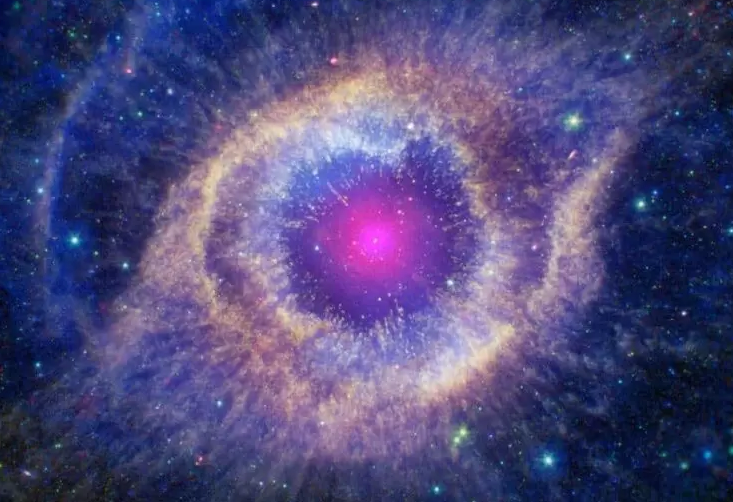
\includegraphics[scale=.4]{img/nebhelix.png}

    {\footnotesize Nebulosa Hélix, concepção artística baseada em dados 
    observacionais - Fonte: NASA}
\end{center}

\section{Introdução}
A Física é uma das Ciências Naturais mais fundamentais que existem; por 
fundamental me refiro ao nível de detalhamento de seu objeto de estudo. Enquanto 
a Química se ocupa "principalmente" das transformações da matéria em nível 
molecular  - quando a agregação das partículas fundamentais que compõem 
a matéria já é extremamente complexa - a Biologia, se ocupa principalmente dos 
organismos sua complexidade e relações - quando a organização molecular se dá 
de maneira tal que pode ser caracterizada como vida. A Física, por outro lado, se
debruça sobre os entes que permitem tais estruturações e vai além; extrapola 
suas inferência para explicar tudo o mais que nos rodeia, a começar do tempo e o
espaço, a matéria, seus distintos estados de agregação, as forças e relações 
quânticas que permitem suas transformações, sua aglutinação gravitacional e a 
formação dos corpos celestes, o próprio ciclo de vida dos elementos componentes
da matéria, constantemente fundidos e destruídos no coração de estrelas jovens e 
velhas, a organização e complexidade das galáxias e o cosmos.

Embora o ser humano seja naturalmente um animal questionador, essa evolução 
científica só foi possível graças a sua capacidade de observar algo de forma 
sistemática, registrá-lo e organizá-lo sistematicamente, de modo tal que o permita
sugerir inferências fundamentadas sobre o observado, questionar o observado e 
buscar respostas consistentes. 

Ao longo da história, as mentes mais curiosas da humanidade fizeram esse 
percurso de construção do conhecimento de muitas formas distintas e não 
lineares. Alguns de forma mais consistentes, outros menos; variações daquilo que
atualmente chamamos \emph{Método Científico}, um conjunto de regras por meio
das quais podemos construir novos conhecimentos de uma forma satisfatoriamente 
confiável. 

Ainda que, o Método Científico seja quase sempre atribuído a Isaac Newton, ou as
vezes a Galileu Galilei, sua criação não pode ser de fato atribuída a um único 
autor. O pensamento greco-ocidental, os lastros históricos do conhecimento 
científico de egípcios, sumérios e mesopotâmicos, o pensamento filosófico 
racionalista e determinista e mesmo contribuições recentes como a Teoria da 
Complexidade de Edigar Morin, foram fundamentais para compor a complexidade e o
nível de especialidade e precisão da Ciência moderna.

No entanto, a despeito de todo o arcabouço conceitual por trás do método, é 
possível sugerir que o átomo do método científico provavelmente seja a 
\emph{medida}. 

\section{Medidas Físicas}
Na Física, a ação de medir deve ser entendida como o ato de se determinar um 
valor \textbf{satisfatóriamente preciso} para uma \emph{grandeza física}.

Note que na definição anterior, dois conceitos foram introduzidos:
\begin{itemize}
    \item[\emph{i)}] o conceito de precisão satisfatória;
    \item[\emph{ii)}] e o conceito de grandeza física
\end{itemize}

O primeiro deles está associado a impossibilidade de se medir com precisão total
o valor de uma grandeza. Em outras palavras \emph{é impossível determinar o 
valor verdadeiro de uma grandeza física.} 

Esta impossibilidade se deve ao fato de que medir algo significa compará-lo com
um determinado padrão. Quando se mede a distância entre duas cidades, o que se 
faz é comparar o espaço entre elas (medido segundo algum critério previamente
determinado, como distância rodoviária ou geodésica) com o padrão quilômetro, 
por exemplo. Logo se quantifica a distância de interesse como múltipla ou 
submúltipla deste padrão previamente estabelecido.

O próprio quilômetro ($km$) é na verdade um múltiplo de uma unidade fundamental 
do Sistema Internacional de Unidades (SI), o metro ($m$). Ainda que exista uma 
definição histórica bastante curiosa para essa grandeza \footnote{Pesquise pela 
"históriado metro" para saber mais}, fisicamente, a unidade métrica é aceita 
como a distância percorrida pela luz em uma fração de tempo igual a 
$1/299 792 458$ segundos. A propósito, a unidade de tempo segundos ($s$) também 
é uma unidade fundamental do SI. 

Deste modo, medir a distância entre duas cidades, significa comparar tal
distância a um conjunto de unidades quilométricas linearmente justapostas a que
dá-se o nome de "escala quilométrica". Uma medida inteira nesta escala hipotética
está condicionado, ao fato de que os pontos que marcam as limites da distância 
medida, coincidam com os extremos de cada unidade quilométrica da escala, medida
esta cuja a probabilidade de ocorrência é baixíssima já que a cada um quilômetro
apenas um ponto atende a essa condição. 

Par descrever qualquer outra medida que não seja inteira, recorre-se aos 
submúltiplos do escala original, o metro por exemplo, \emph{a o que se denomina 
aumento de resolução}. Deste modo a escala quilométrica passa a ser subdividida 
em 1000 partes iguais,  cada qual com 1 $m$ de extensão. No entanto, retorna-se 
certamente na mesma dificuldade de medida, já que a cada metro apenas um ponto 
é capaz de expressar um valor inteiro de medida nessa escala. Medidas não 
inteiras poderiam ser expressas como a centésima parte do metro o centímetro 
($cm$) e em seguida milímetros e assim sucessivamente \emph{ad infinitum}. 

Como se vê, a redução da escala incrementa a precisão de uma medida apenas até
certo nível, já que independentemente daquela utilizada, o problema da 
indeterminação do valor absoluto da medida se mantém, considerando que apenas
o conhecimento de um determinado ponto dentre outros infinitos atenderia essa 
premissa. Além disto, o incrementos sucessivos na resolução da escala, 
simultaneamente potencializa a questão da \emph{acuidade}, que é nível de 
capacidade que um determinado sensor - um ser humano usando o sentido da visão, 
por exemplo - possui de perceber a distinção entre múltiplas medidas. Donde se
chega a ideia de \emph{precisão satisfatória} para a medida sendo realizada. 
\newline 
\begin{myboxed}
    \textbf{IMPORTANTE:}
    \emph{
        Deve-se estabelecer de forma planejada e antecipada, o nível de precisão 
        desejado para uma medida, e só então selecionar o instrumento e 
        a metodologia ideal para a tomada desta.
    }
\end{myboxed}

\subsection{Incerteza de Medidas}
Obviamente, quando se estabelece uma precisão limite, não se pode apenas
desprezar a imprecisão associada, de modo tal que é preciso tratar a 
\textbf{\emph{incerteza}} ($\sigma$) associada à medida. Assim para a expressão 
correta de uma medida, é preciso informar simultaneamente o valor da leitura e 
esse valor de incerteza. 

A incerteza representa o intervalo de confiança de uma leitura através de um 
intervalo finito e não nulo representado nas formas das Equações 
\ref{Eq:med_incert_simetrica} e \ref{Eq:med_incert_assimetrica}

\begin{equation}
    m = M \pm \sigma
    \label{Eq:med_incert_simetrica}
\end{equation}
\begin{equation}
    m = M^{+\sigma'_{M_+}}_{-\sigma''_{M_-}}
    \label{Eq:med_incert_assimetrica}
\end{equation}

A Equação \ref{Eq:med_incert_simetrica} representa a incerteza simétrica em 
torno da leitura ($M$), ao passo que a Equação \ref{Eq:med_incert_assimetrica}
representa a incerteza assimétrica em torno de $M$. Ou seja $M$ pode variar 
entre $M + \sigma$ e $M - \sigma$ na Equação \ref{Eq:med_incert_simetrica} e 
$M + \sigma'$ e $M - \sigma''$ na Equação \ref{Eq:med_incert_assimetrica}.

São muitos os métodos para o cálculo de $\sigma$, para a avaliação da precisão 
e seleção do número de algarismos significativos, e dependem, dentre outras 
coisas, do instrumento utilizado, da metodologia e do número de fontes de erros.
Os detalhes deste tipo de análise merecem considerações mais pormenorizadas e 
uma discussão mais elaborada, e só serão tratados desta forma em outra obra 
complementar a essa. 

No entanto, algumas convenções simples podem ser adotadas.

\subsubsection{Convenções sobre incertezas e algarismos significativos}
Algarismos significativos \emph{são os dígitos numéricos de um valor que 
possuem significado}, exatamente por isso podem ser utilizados para se 
representar, dentre outras coisas, estimativas da incerteza de uma medida.

Suponha uma régua semelhante à da Figura \ref{Img:reguaescolar}, 
graduada em milímetros ($mm$). Ao ser usada para medir o 
objeto, a leitura obtida é certamente 63 $mm$, porém há alguma 
dúvida sobre o comprimento do objeto que se estende para além deste ponto. 

\begin{staticfigure}
    \centering
    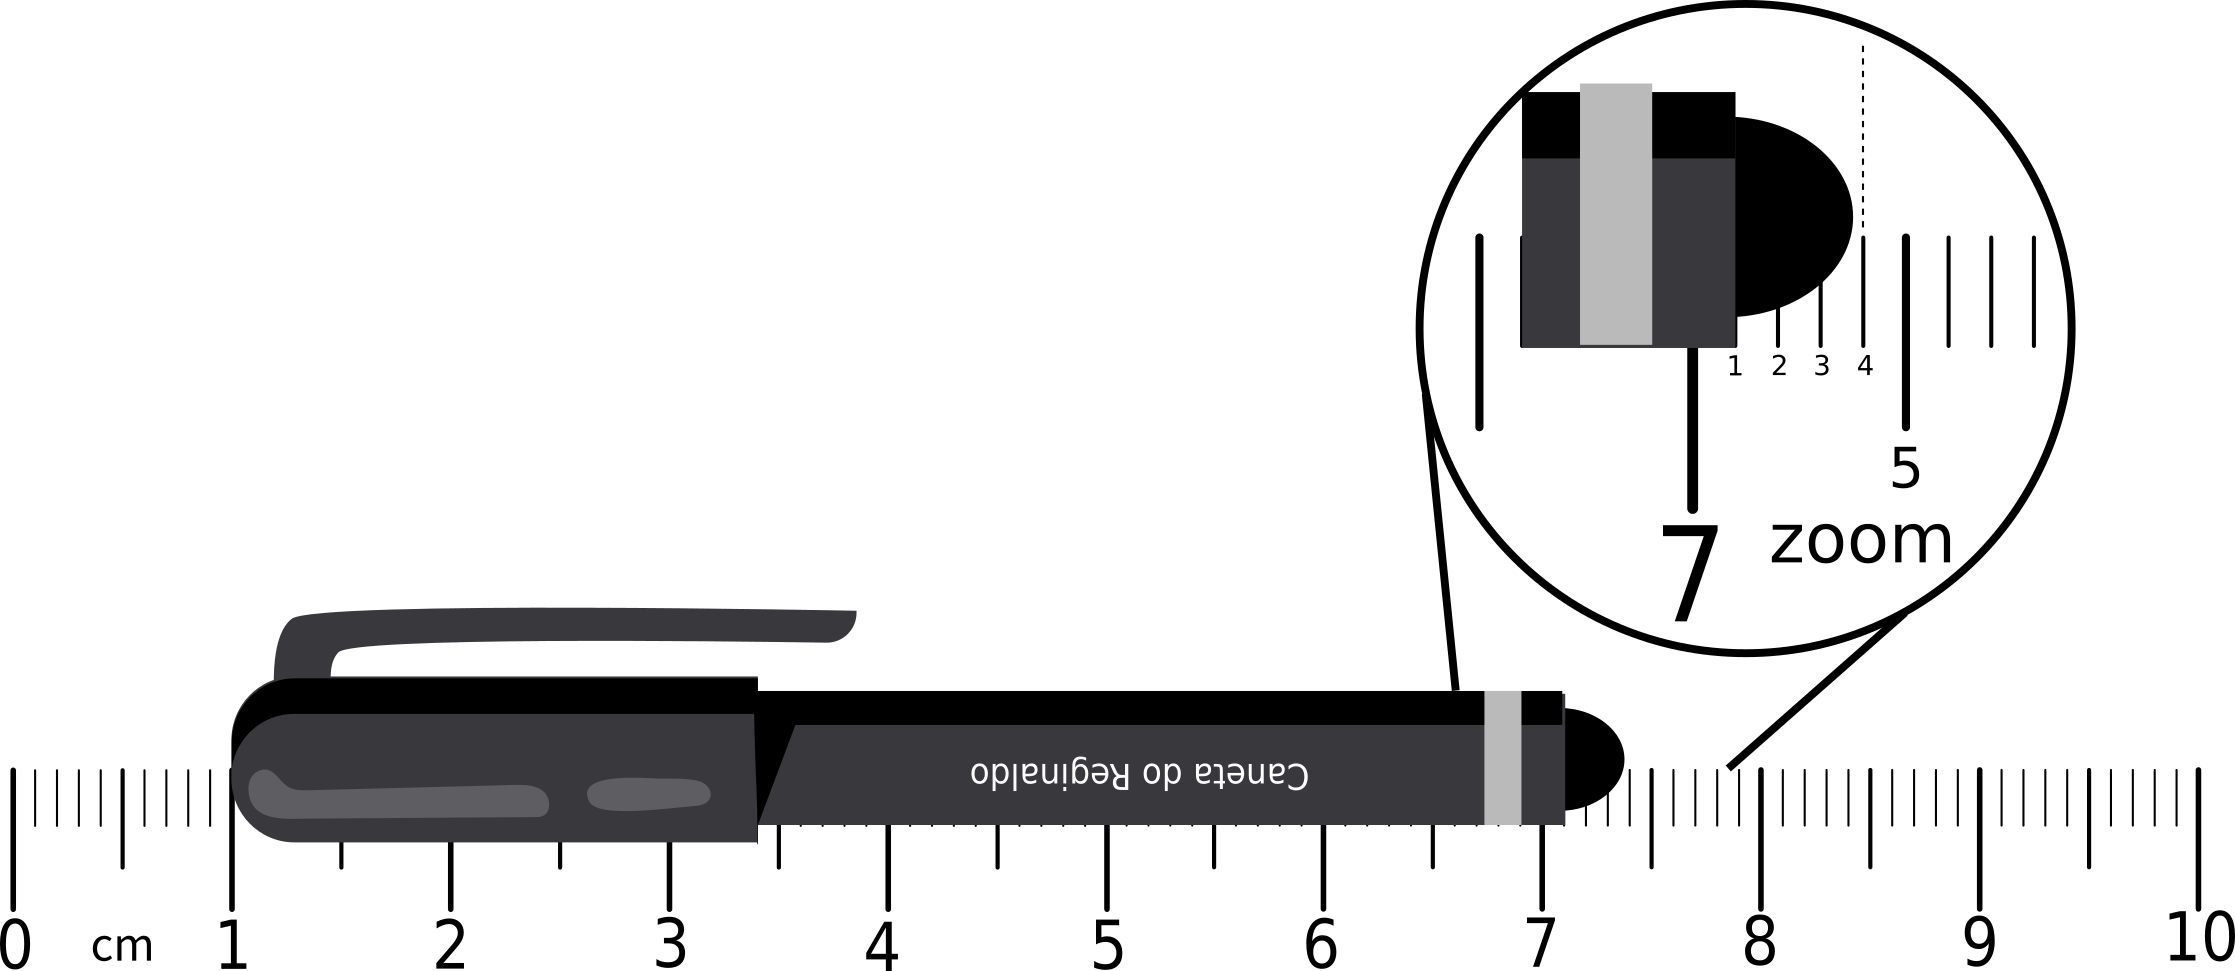
\includegraphics[scale=.45]{img/reguaescolar.png}
    \caption{\footnotesize Régua graduada.}
    \label{Img:reguaescolar}
\end{staticfigure}

Observando mais atentamente a região de \emph{zoom} na imagem, é possível 
observar que a extremidade da caneta está além do terceiro milímetro após a 
marcação de 7 $cm$ na escala. Alguns avaliarão essa medida residual como 
como $7/10 \: mm$, provavelmente a maioria como $8/10 \: mm$ e
alguns ainda avaliarão como $9/10 \: mm$. De fato, 63,7 $mm$, 63,8 $mm$ e 
63,9 $mm$ \textbf{são todas medidas válidas, igualmente certas e igualmente 
erradas}.

A leitura 63 corresponde ao valor de $M$ na Equação 
\ref{Eq:med_incert_simetrica}, mas qual a incerteza dessa medida ? 

Em instrumentos analógicos, como é o caso da escala graduada, a convenção mais 
comum adota a incerteza como sendo igual a metade da \textbf{precisão} do 
instrumento. A escala da Figura \ref{Img:reguaescolar} tem precisão de 1 $mm$, 
portanto, a incerteza de medidas em escalas como essa é de 0,5 $mm$. 
Considerando um leiturista que sugerisse 63,8 $mm$ para o tamanho da caneta, 
o valor da medida seria $m = 63,8 \pm 0,5$ $mm$.

Na leitura em questão a convenção demonstrada na Figura \ref{Img:algsign} é 
adotada para a identificação dos algarismos significativos. 

\begin{staticfigure}
    \centering
    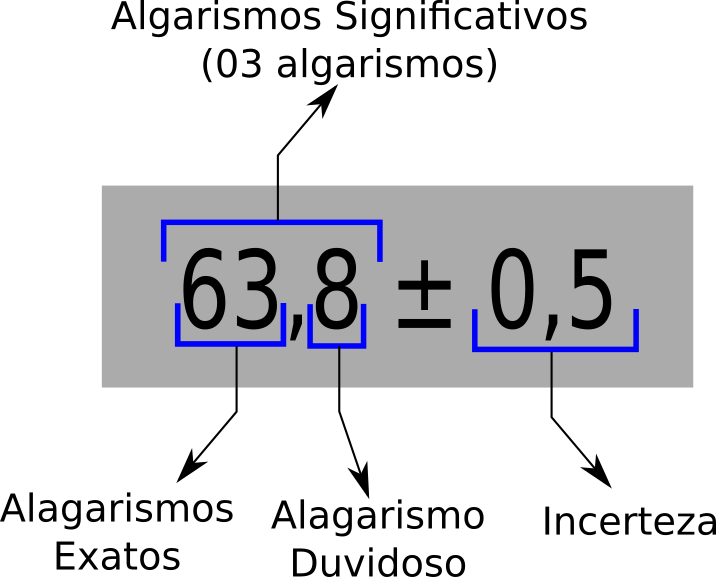
\includegraphics[scale=.55]{img/algarismossig.png}
    \caption{\footnotesize Algarismos de uma leitura.}
    \label{Img:algsign}
\end{staticfigure}

Algarismos exatos são aqueles que se pode determinar com certeza absoluta na 
leitura da escala, já o algarismo duvidoso, será sempre aquele que pode 
suscitar dúvida entre diferentes leituristas. Como o algarismo duvidoso 
carrega inexatidão, \emph{não faz sentido que qualquer leitura possua mais do que 
apenas um algarismo deste tipo}.

Outra convenção importante que geralmente é adotada na falta de algo mais 
preciso, é a forma de determinação da incerteza de uma medida na qual este 
valor não foi explicitamente declarado. Nestes casos, \emph{é comum se adotar a 
incerteza como sendo a metade do valor unitário do menor alagarismo exato}.

\begin{myboxed}
    \textbf{IMPORTANTE:}

    \emph{
    1. Qualquer medida de uma determinada grandeza deve possuir apenas um 
    algarismo duvidoso.
    }

    \emph{
    2. A incerteza de medidas para as quais este valor não foi explicitamente 
    declarado, deve ser assumida como sendo igual à metade do valor unitário do
    menor algarismo significativo exato.
    }
\end{myboxed}

\subsubsection{O problema do algarismo zero (0)}
Zeros que são colocados em um número para posicionar o separador decimal, jamais
devem considerados algarismos significativos. Estes casos são melhores 
identificados na composição de medidas expressas em unidades de medida 
diferentes daquelas dos instrumentos em que foram determinadas.

Suponha, por exemplo, uma balança comercial com precisão de 0,1 quilogramas 
($kg$), que tenha feito uma leitura de 2,5 $kg$. Quando este valor é expresso em
gramas - uma unidade de medida distinta daquela original da balança -, então a 
leitura ficaria 2500 gramas ($g$). Note que no número 2500 os zeros a direita, 
não tem significado pois a balança não possui tal precisão, portanto não são 
significativos e só existem para possibilitar a ocorrência do ponto decimal 
em uma posição correspondente a unidade grama.

De forma semelhante, se uma balança graduada em gramas mede 20 $g$ e o 
usuário, desejando expressar esse valor em $kg$ o escreve como 0,020 $kg$, os 
zeros a esquerda não são significativos, pois só foram introduzidos para 
possibilitarem a colocação do separador decimal na casa deciaml correspondente 
à unidade de medida de massa desejada. Este tipo de técnica é bastante comum na 
Física, quando se precisa compatibilizar diferentes unidades de medida de uma 
mesma grandeza, ou se operar com grandezas distintas compondo uma unidade 
derivada desejada, ou mesmo para a compatibilização de unidades com constantes 
físicas. 

Para evitar a dificuldades no acompanhamento dos algarismos significativos, é 
bastante recomendável que as medidas e constantes físicas sejam expressas como 
potências de 10 em Notação Científica. 

\subsubsection{Notação Científica}
A natação científica é uma recurso de representação de valores por meio de 
potências de dez ($10^{n}$) multiplicadas pela mantissa ($\mathcal{M}$) do valor
 que se deseja representar somada à incerteza deste valor, conforme mostrado pela 
 Equação \ref{Eq:pot_dez}.

 \begin{equation}
     m = (\mathcal{M} \pm \sigma) \cdot 10^n
     \label{Eq:pot_dez}
 \end{equation}

É também convencionado que o valor de $\mathcal{M}$ deve estar no intervalo 
determinado por $1 \leq \mathcal{M} < 10$.

Para compreender melhor o uso do recurso, vamos expressar a leitura da régua 
para o tamanho da caneta em notação científica. Como a medida foi de 
$63,8 \pm 0,5 \: mm$, deve-se multiplicar o valor por $10^{-1}$ para que a 
mantissa esteja entre $1 \leq \mathcal{M} < 10$.

\begin{myboxed}
    \textbf{SEÇÃO DE CÁLCULOS:}

    $
        (63,8 \pm 0,5) \cdot 10^{-1} = (6,38 \pm 0,05) \cdot 10^{-1}
    $
\end{myboxed}

Neste caso, a vantagem do uso de notação científica não é tão aparente, porém, 
no exemplo da seção anterior quando o significado dos zeros na leitura 
$2500 \: g$ foi discutido, a forma de $\mathcal{M}$ indica exatamente o número 
de algarismos significativos no valor.

\begin{myboxed}
    \textbf{SEÇÃO DE CÁLCULOS:}

    $
        (2500 \pm 100) \cdot 10^{-3} \: g = (2,5 \pm 0,1) \cdot 10^{-3} \: g
    $
\end{myboxed}

É possível notar que a mantissa possui exatamente dois algarismos 
significativos, além disso, deve ser observado que neste instrumento em 
específico a incerteza foi assumida como sendo de $100 \: g$. \emph{Em 
instrumentos digitais a incerteza é fornecida pelo fabricante ou convencionada 
como sendo sua resolução}.

\subsubsection{Algarismos Significativos nas Operações Matemáticas 
Básicas}

Quando grandezas são operadas matematicamente deve-se determinar uma convenção 
para o tratamento do número de algarismos significativos e incertezas de 
medidas. Os métodos de tratamento da propagação das incertezas através das 
operações matemáticas são um pouco mais complexos e não serão tratados neste 
tópico introdutório. Todavia, as convenções para o cuidado com o número de 
algarismos significativos são bastante simples conforme pode ser visto na lista
abaixo.

\begin{myboxed}
    \textbf{Convenções para determinação do número de algarismos significativos 
    nas operações matemáticas básicas.}

    \begin{enumerate}
        \item \textbf{SOMA E SUBTRAÇÃO:} O número de \emph{casas decimais} no 
        resultado deve ser igual ao número da menor quantidade de casas dentre 
        aquelas presentes nos termos da operação.
        \item \textbf{MULTIPLICAÇÃO E DIVISÃO:} O número de \emph{algarismos 
        significativos} no resultado deve ser igual ao número da menor 
        quantidade de algarismos significativos dentre aqueles presentes nos 
        termos da operação.
        \item \textbf{ESTIMATIVAS:} Todos os resultados estimados devem possuir
        apenas um algarismo significativo, segundo sua órdem de grandeza. 
    \end{enumerate}
\end{myboxed}

Quando arredondamento se fizerem necessários para o atendimento às regras 
anteriores, então a seguinte convenção deve ser utilizada.

\begin{myboxed}
    \textbf{Regras para arredondamento}

    Após a seleção do total de dígitos conservados - aqueles que parmanecerão no 
    valor - segundo as regras de determinação do número de algarismos 
    significativos, deve-se verificar se:

    \begin{itemize}
        \item o primeiro algarismo abandonado for maior que 5, ou sendo 5 e 
        o seguinte qualquer que não seja 0, o último 
        dígito conservado deve ser acrescido de uma unidade  
        (e.g. $1,7|6 \rightarrow 1,8| $ ou $1,7|51 \rightarrow 1,8| $); 
        \item o primeiro algarismo abandonado for menor que 5, o último 
        dígito conservado não deve ser alterado 
        (e.g. $1,7|3 \rightarrow 1,7| $);
        \item  o primeiro algarismo abandonado for igual a 5 seguido de um 
        dígito zero, o último dígito conservado deve ser acrescido 
        de uma unidade, se for ímpar, e mantido, se for par.
        (e.g. $ 1,7|51 \rightarrow 1,8| $ ou $ 1,6|51 \rightarrow 1,6| $); 
    \end{itemize}
\end{myboxed}

\subsubsection{Ordens de Grandezas e Estimastivas}

\begin{flushright}
    A \emph{Via-Láctea} é uma galáxia espiral com pouco mais \\
    de $10^5$ anos luz de diâmetro, idade de $10^{10}$ anos \\
    terrestres e $10^{11}$ estrelas vivas. 
\end{flushright}

Ao ler o texto anterior, não é difícil inferir que os dados informados são todos
\textbf{estimativas} dos respectivos valores reais, impossíveis de serem 
determinados precisamente no atual estágio de desenvolvimento científico. 

Os valores usados para representar as grandezas mencionadas são todos exemplos de 
estimativas dadas como \textbf{ordens de grandeza}. 

Uma ordem de grandeza, é uma potência de dez (\emph{atenção para não confundir
o conceito com o de notação científica}) usada para expressar com confiabiliade 
aceitável, um valor cuja a expressão precisa seja impossível, muito dispendiosa, 
ou desnecessária. \emph{A potência selecionada para este propósito, deve ser a mais
próxima do valor que se está estimando.} 

As dimensões de nossa galáxia, o número de átomos de carbono presentes em um 
organismo vivo, o número de elétrons livres por $m^3$ em um condutor elétrico, 
são todos exemplos de grandezas que podem ser satisfatoriamente representadas 
apenas por uma órdem de grandeza. 

Vejamos um exemplo.

\begin{myboxed}
    \textbf{EXEMPLO - Estimando o número de átomos de carbono no corpo humano.}

    No livro 
    \emph{What Do You Think You Are? The science of what makes you you}, de 
    Brian Clegg, o autor estima o fração mássica média de átomos de carbono no 
    organismo humano como algo próximo de 18\%. 

    Sabendo disto, estime a ordem de grandeza do número de átomos de carbono 
    em um ser humano com massa de 70 kg.

    \textbf{SOLUÇÃO:}

    Se 18\% dos 70 kg da massa corpórea na situação proposta forem átomos de 
    carbono ($C$), então tem-se uma massa de:
    
    $$
        m_C = 70 \cdot 0,18 \approx 13 kg
    $$

    Considerando a massa do elemento C, dada a abundância isotópica, como de 
    aproximadamente $12 \: g.mol^{-1}$. Então em $1,3 \cdot 10^4 \: g$
    \emph{
        (Note aqui a utilização da notação científica para adequação do número de
        algarismos significativos.)
    }
    tem-se:

    $$ 
        M_{molar} = \frac{m}{N_{mols}} \rightarrow 
        12 = \frac{1,3 \cdot 10^4}{N_{mols}} \rightarrow 
        N_{mols} \approx 1,1 \cdot 10^3 mols
    $$

    Agora considerando a constante de Avogadro ($N_A$) como $6,0 \cdot 10^{23}$, podemos
    determinar o número de átomos $N_C$.

    $$
        N_C = {N_{mols}}\cdot{N_A} = {1,1 \cdot 10^3}\cdot{6,0 \cdot 10^{23}} 
        \rightarrow N_C \approx 6,6 \cdot 10^{26}  \approx 10^{27} 
        \text{ átomos de carbono}.
    $$
 
\end{myboxed}

Alguns valores como 5, 50, 500... geralmente costumam gerar alguma confusão 
quando precisam ser expressos como ordens de grandeza, no entanto a confusão é 
apenas aparente. Note na sequência abaixo que o número cinco não é um ponto 
equidistante às potências de 10 mais próximas, mas sim o  valor 5,5.

$$
    ...10^0, 2, 3, 4, \text{\LARGE 5}, 6, 7, 8, 9, 10^1...
$$

Deste modo, utilizaremos como critério de seleção da potência de dez a seguinte
regra:

\begin{myboxed}
    \textbf{Regras para a seleção da potência de dez em estimativas de órdens
    de grandeza.}

    Valores que quando expressos na forma de notação científica sejam menores
    5,5 terão ordem de grandeza igual à potência de dez da notação, do contrário
    terão ordem de grandeza igual à potência de dez imediatamente superior.
\end{myboxed}


\label{lastpage}
\end{document}